


\chapter{Multi-channel geometrical effects in tunnel ionization}
\label{chap:multi-channel}
This chapter examines the mechanism of correlation-assisted tunnelling ionization, as expressed in the correlation-driven term examined in section~\ref{sec:correlation-driven-ionization}. Here we examine the correlation-assisted contribution in terms of its geometrical features, looking for qualitative traces that can help establish, beyond pure ionization rates, the role of the correlation-assisted mechanism in tunnel ionization. We find that the direct and correlation-driven terms can have different geometrical structures, which could then be used as a way to demonstrate the presence of correlation effects in strong-field ionization. 

Some of the material in this chapter has appeared previously in reference
\begin{enumerate}
\item[{\hypersetup{citecolor=black}\citealp{Pisanty_momentum_transfers_2014}}.]
\textsc{E.~Pisanty and M.~Ivanov}.
\newblock Momentum transfers in correlation-assisted
  tunneling.
\newblock \href{http://dx.doi.org/10.1103/PhysRevA.89.043416}{
          \emph{Phys. Rev. A} \textbf{89} no.~4, p.~043\,416 (2014)}.
\newblock \href{http://arxiv.org/abs/1309.4765}{{arXiv}:1309.4765}.
\end{enumerate}
\noindent
and in the author's MRes report,
\begin{enumerate}
\item[{\hypersetup{citecolor=black}\citealp{MResReport}}.]
\textsc{E.~Pisanty}.
\newblock \emph{Under-the-barrier electron-ion interaction during tunnel
  ionization}. 
  \href{http://www3.imperial.ac.uk/controlledquantumdynamics/people/students/cohortthree/emiliopisantyalatorre }{
\newblock {MRes} report, Imperial College London (2012)}.
\newblock \href{http://arxiv.org/abs/1307.7329}{arXiv:1307.7329}.
\end{enumerate}
\noindent
This chapter mostly follows the lines of \citer{Pisanty_momentum_transfers_2014}.



\section{Electron correlation in strong-field ionization}
Throughout much of its history, and for most of its applications, strong-field physics can essentially be understood as a single-electron game, mostly because the post-ionization part of the dynamics, with the electron at the mercy of the radiation field, is at heart a single-electron phenomenon. 

However, this is at odds with the rest of atomic physics, which breaks down completely if electron correlation and exchange are not included as core parts of the theory. Within photoionization alone, for example, multi-electron effects appear in a multitude of phenomena, which include autoionizing states~\cite{fano_resonances_1961}, giant resonances~\cite{amusia_giant-resonances_2000}, shake-off~\cite{schneider_knockout-shakeoff_2002}, shake-up~\cite{matveev_shakeup_1982}, Auger and frustrated Auger decay~\cite{cooper_auger-decay_2013}, interatomic Coulomb decay~\cite{averbukh_ICD_2004}, and ultrafast correlation-driven hole migration~\cite{cederbaum_ultrafast-charge-migration_1999, kuleff_hole-migration_2005} among many others. These correlation-driven mechanisms often leave clear traces that can be used to identify them, but the distinction between different mechanisms can also be blurry, as in the case of separating the contributions of shake-up and post-ionization interaction~\cite{hino_perturbation-theory-diagrams-gauge_1993}.


Strong-field ionization, however, mostly works as a single-electron theory, as attested by the wide success of the Strong-Field Approximation in its many forms, the overwhelming majority of which are single-electron theories, or include the effect of the ionic electrons at the self-consistent-field level~\cite{pfeiffer_self-consistent-effects_2012}. The inclusion of multielectron effects beyond this level was triggered by the realization that the molecular ions produced by strong-field ionization are often electronically excited~\cite{zon_tunnelling-excitation_2000, litviniuk_shakeup_2005}, and that these excitations affect all subsequent processes~\cite{smirnova_multielectron-hhg_2009, mairesse_high-harmonic-spectroscopy_2010, torres_molecular-structure-and-dynamics-hhg_2010, haessler_attosecond-imaging_2010, lin_rescattering-self-imaging_2010}. Recent experiments~\cite{boguslavskiy_multielectron-ionization_2012, wen_n2o4-excited-ionization_2008} and \textit{ab initio} simulations~\cite{spanner_one-electron_2009,farrell_strong-field-excited-ionization_2011} confirm that, for molecules in strong fields, electronic excitations during the ionization process are the rule rather than an exception.

Two main mechanisms are responsible for creating an ion in an excited state after optical tunnelling: the laser may remove an electron from a low-lying orbital, leaving the ionic core excited~\cite{zon_tunnelling-excitation_2000, smirnova_multielectron-hhg_2009, mairesse_high-harmonic-spectroscopy_2010, torres_molecular-structure-and-dynamics-hhg_2010, haessler_attosecond-imaging_2010, lin_rescattering-self-imaging_2010, zon_many-electron_1999, zon_many-body_2010, kornev_neon-excited-ionization_2004, kornev_kinetics_2003, kornev_many-body-effects_2003, guehr_hhg-multiple-orbitals_2008}, shown schematically in \reffig{f3-direct-vs-correlated-direct}, or the electron may depart from the highest occupied molecular orbital (HOMO), and subsequently excite the core through a Coulomb interaction. This can happen inside the tunnelling barrier~\cite{walters_correlation-during-tunnelling_2010}, shown in \reffig{f3-direct-vs-correlated-midbarrier}, or after the tunnelling step~\cite{zon_tunnelling-excitation_2000, litviniuk_shakeup_2005}, as shown in \reffig{f3-direct-vs-correlated-postionization}.


\newlength{\figurethreeblwidth}
\setlength{\figurethreeblwidth}{0.28\textwidth}
\begin{figure}[htbp]
  \centering
  \begin{tabular}{ccc}
  (a) & (b) & (c) \\[-2mm]
  \subfigure{
    \label{f3-direct-vs-correlated-direct}
    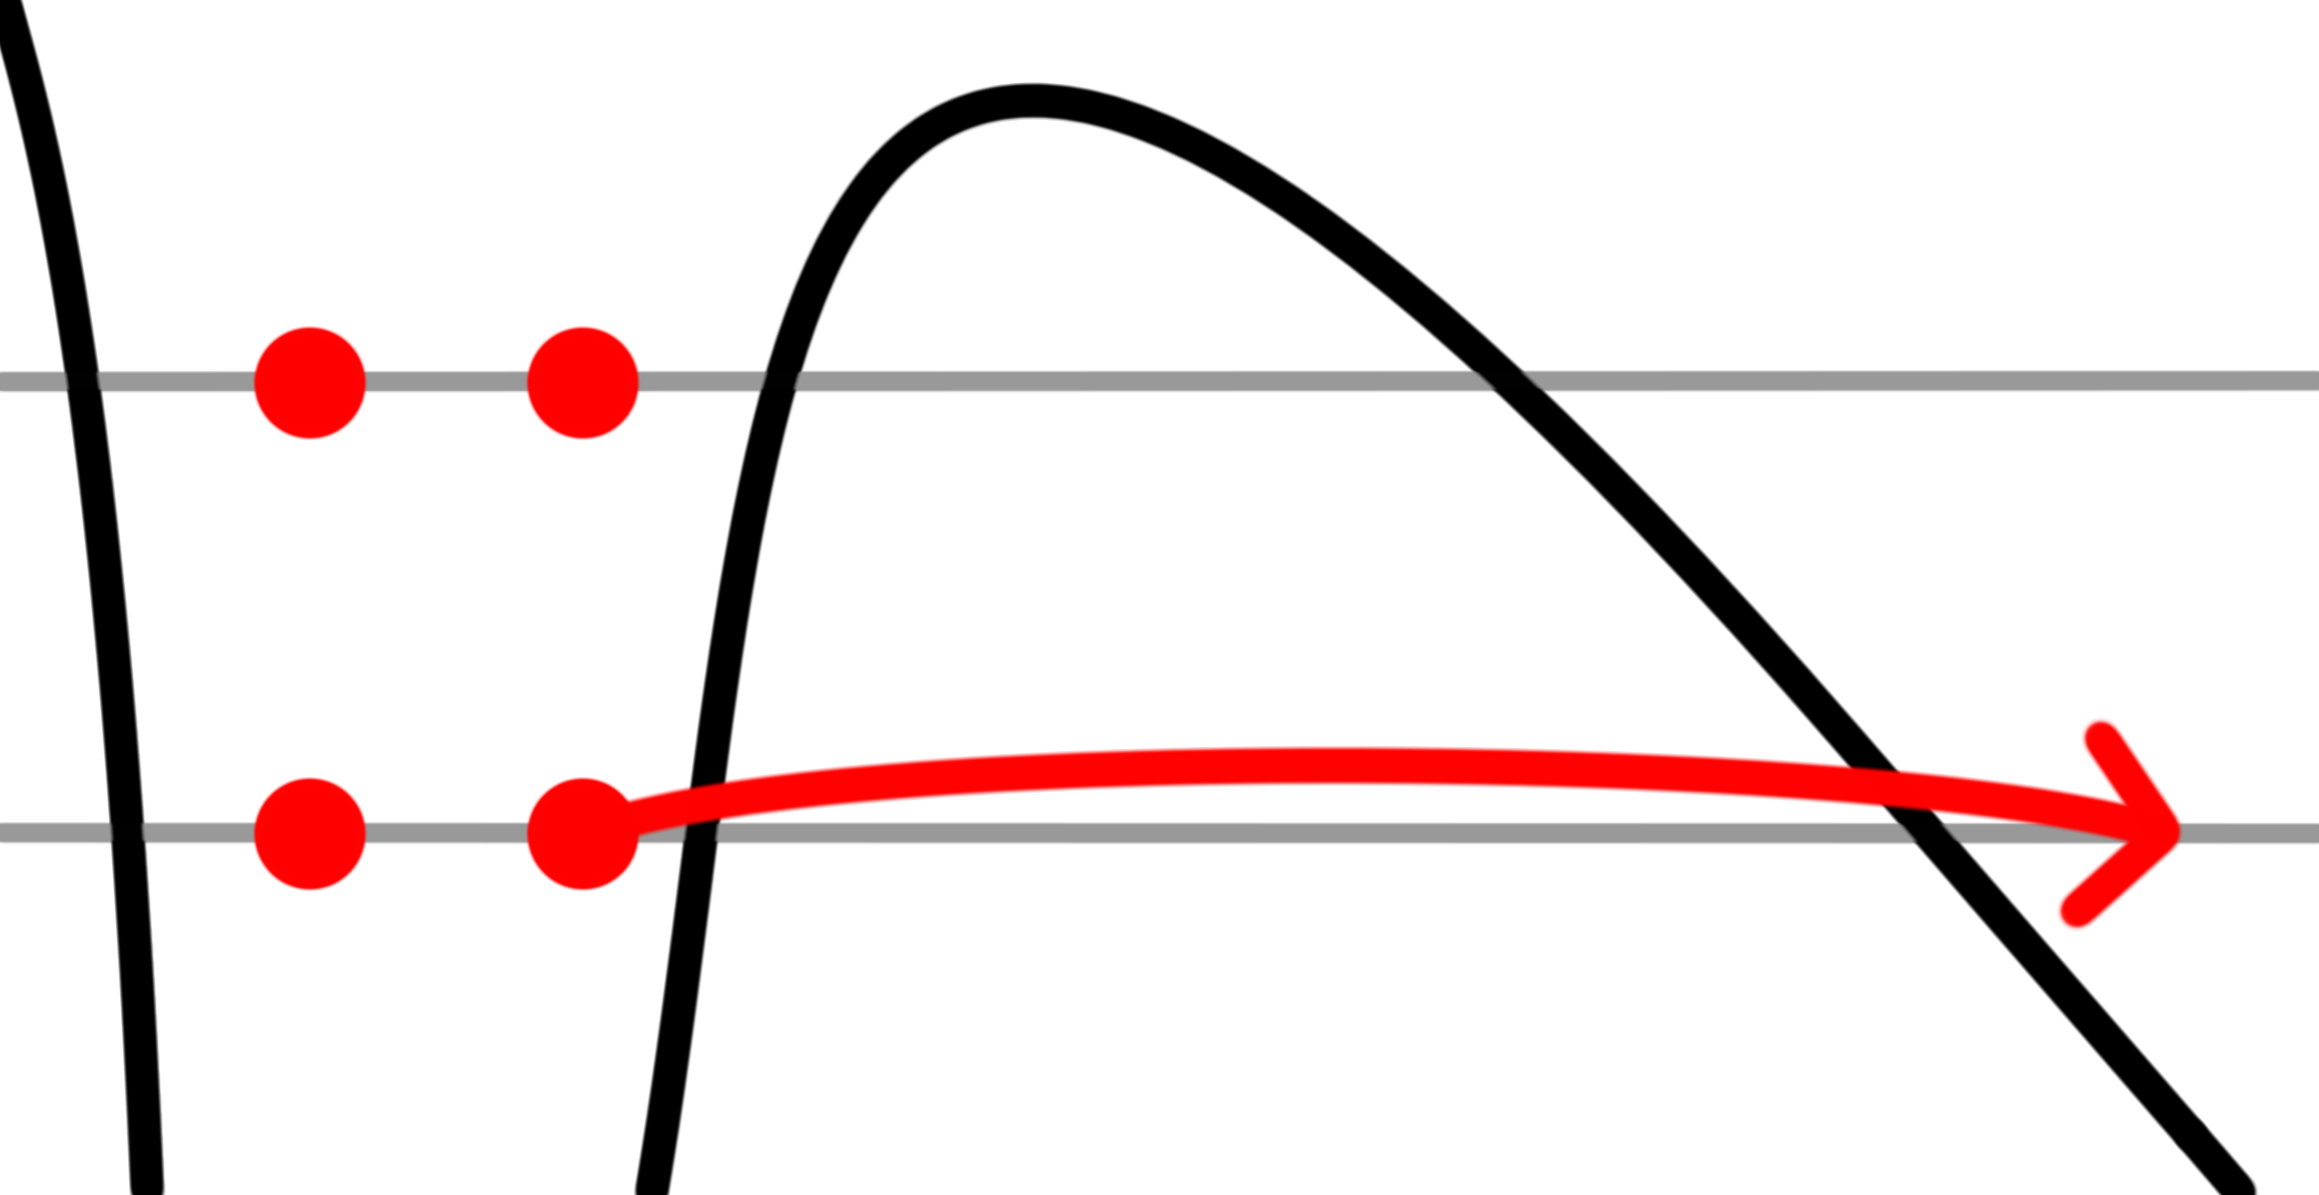
\includegraphics[width=\figurethreeblwidth]{3-Multi-channel/Figures/figure3Ba.png}
  }
  &
  \subfigure{
    \label{f3-direct-vs-correlated-midbarrier}
    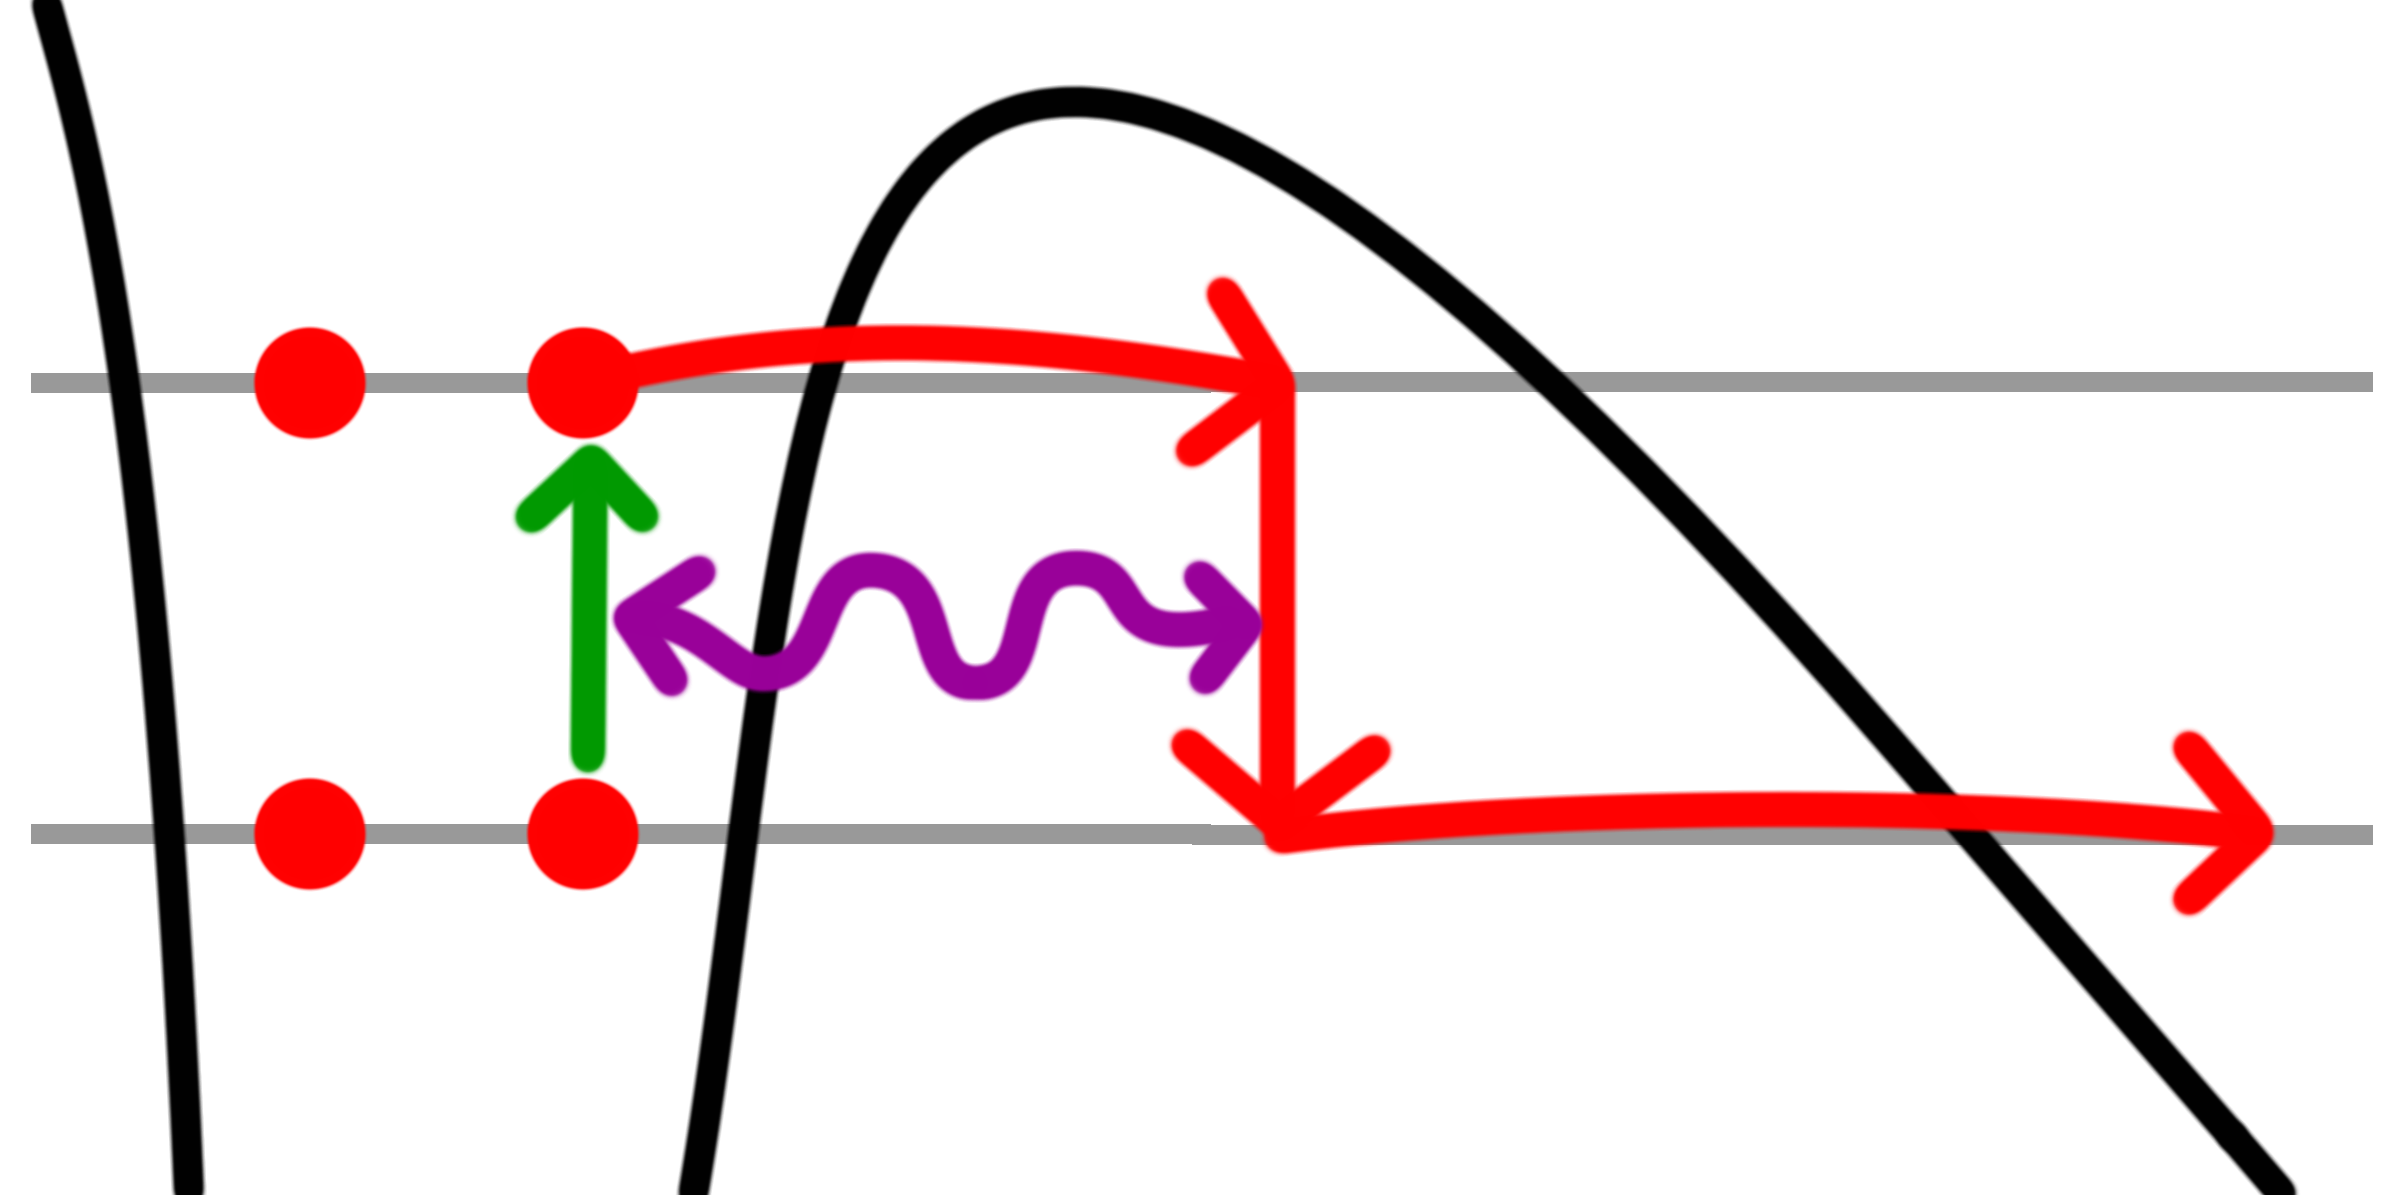
\includegraphics[width=\figurethreeblwidth]{3-Multi-channel/Figures/figure3Bb.png}
  }
  &
  \subfigure{
    \label{f3-direct-vs-correlated-postionization}
    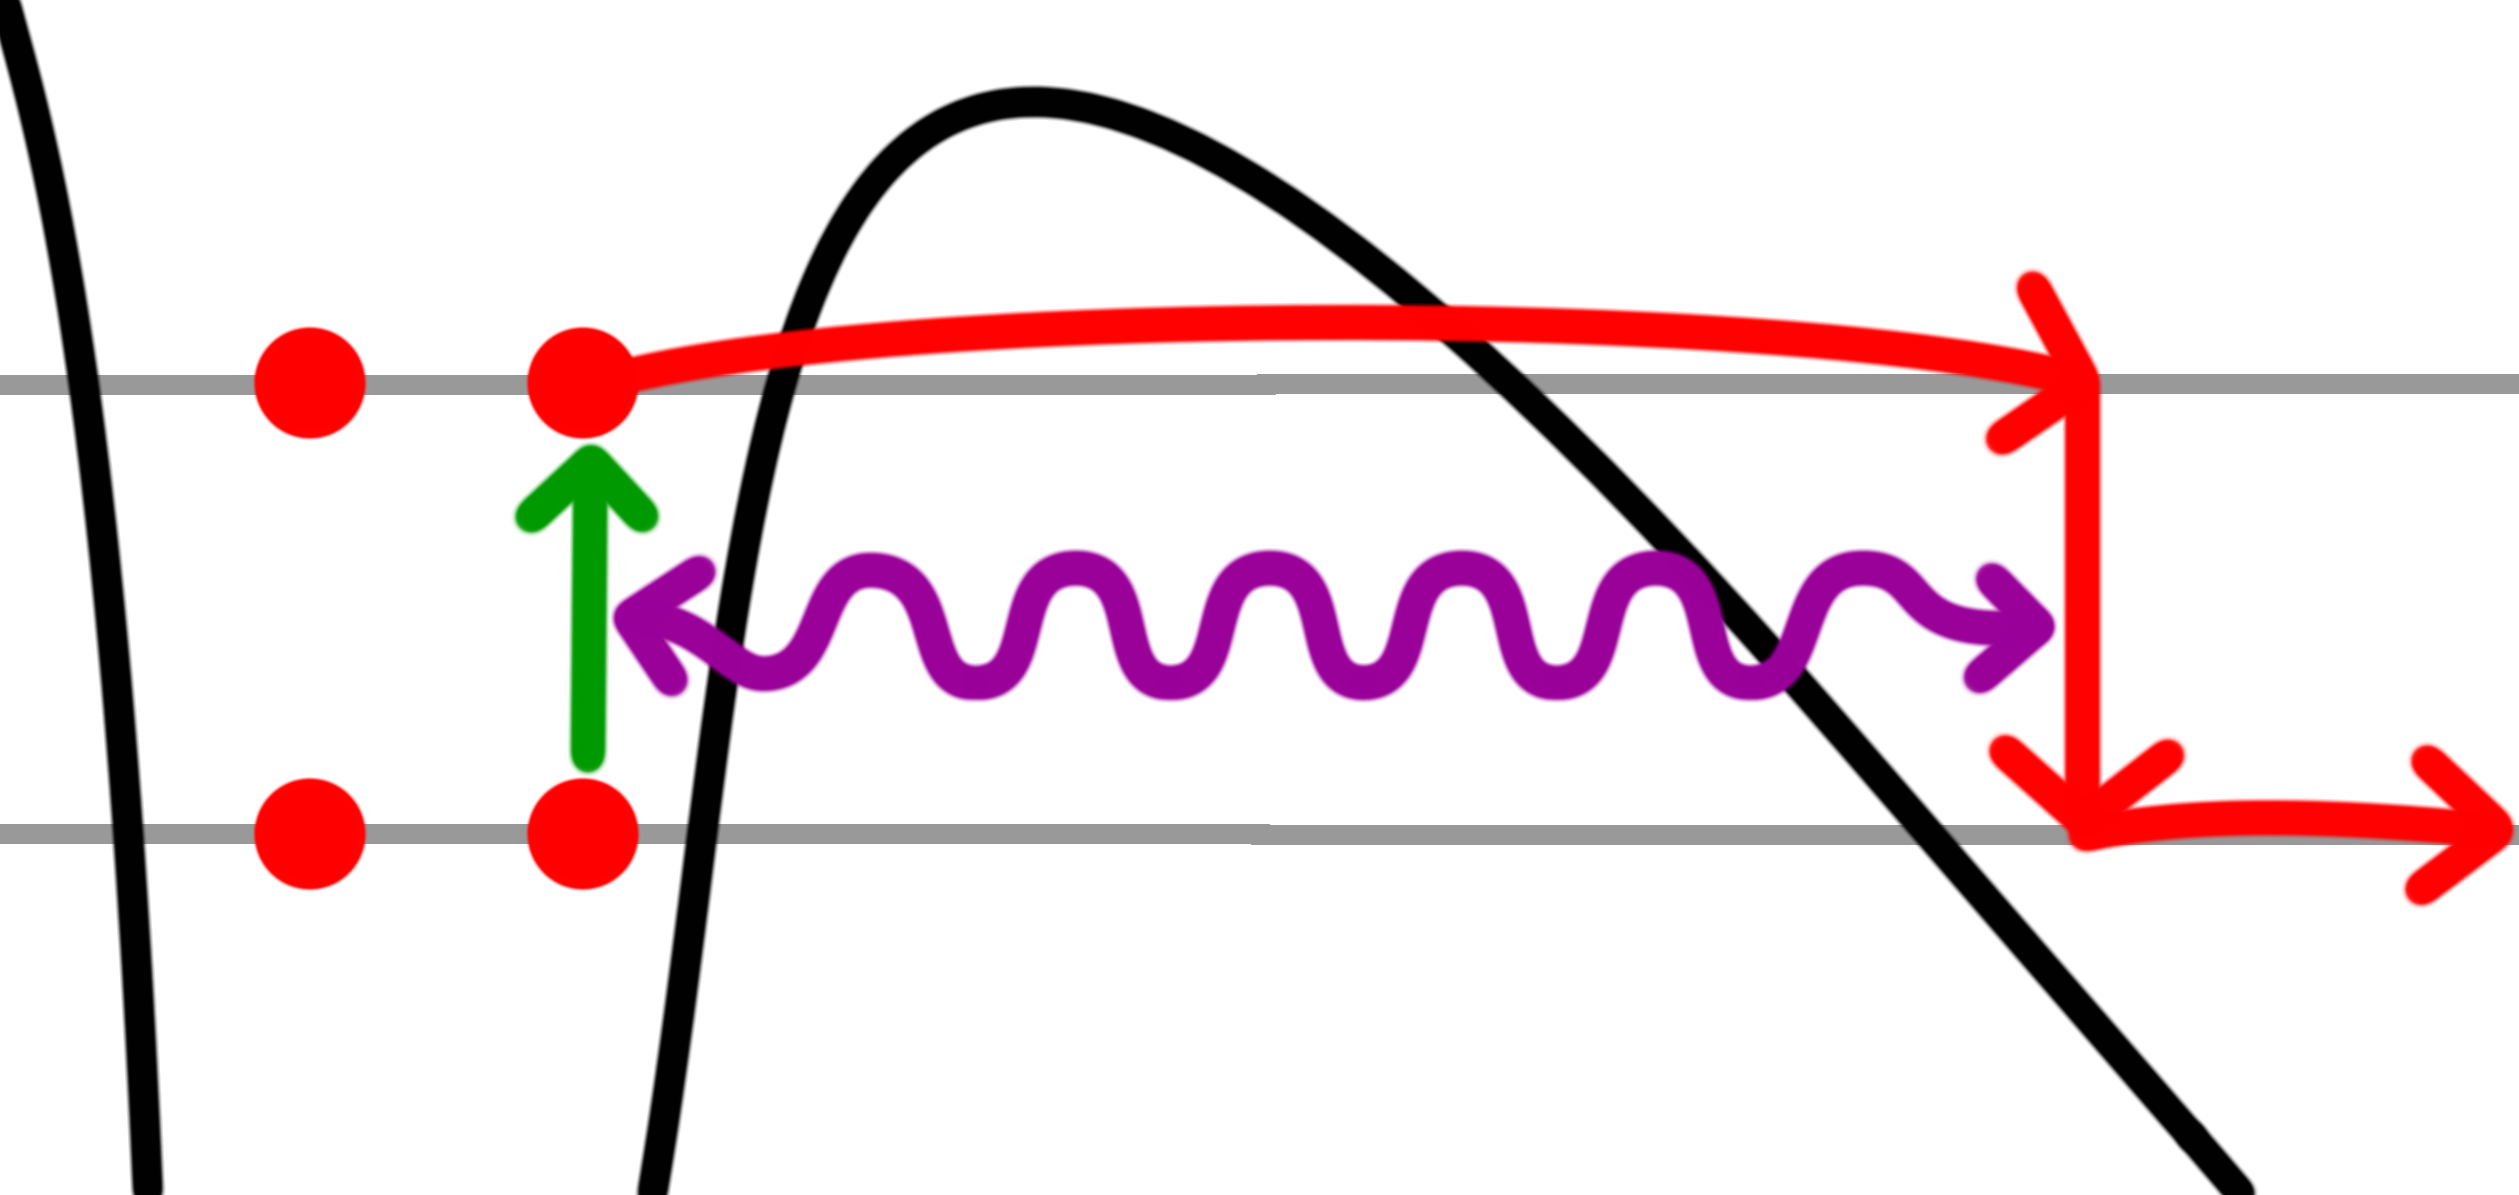
\includegraphics[width=\figurethreeblwidth]{3-Multi-channel/Figures/figure3Bc.png}
  }
  \end{tabular}
  \caption[Three processes that leave the ion excited: direct ionization from a sub-HOMO orbital, or interaction-driven transitions before and after the tunnel exit]{Three possible ionization processes which leave the core excited: the ionized electron may depart from a sub-HOMO orbital \protect\subref{f3-direct-vs-correlated-direct}, or it may depart from HOMO and subsequently interact with the core, either inside the tunnelling barrier~\protect\subref{f3-direct-vs-correlated-midbarrier} or after the ionization step~\protect\subref{f3-direct-vs-correlated-postionization}.
  }
\label{f3-direct-vs-correlated}
\end{figure}



Analyzing strong-field ionization in a way that permits the description of electronic excitations in the ion that is left behind (and, indeed, that allows the photoelectron to return and interact with this excited ion), and to describe it in an analytical form that can help us grasp the physical mechanisms at play, is far from an easy task. Fortunately, though, our ARM theory of photoionization is perfectly capable of handling this, and indeed it was initially developed with this in mind~\cite{ ARM_initial_multielectron}. However, the original ARM implementations only considered the total ionization rates, and these do not readily yield direct, qualitative traces of the multielectron interactions that help shape the tunnelling process.

This chapter looks for such traces in the angular distribution of the photoelectron; we show that the correlation-assisted tunnelling, as shown in Figs.~\ref{f3-direct-vs-correlated-midbarrier} and \subref{f3-direct-vs-correlated-postionization}, produces wavepackets with nontrivial spatial structure as compared with the direct tunnelling of \reffig{f3-direct-vs-correlated-direct}. The correlation-driven structures, then, should interfere with the direct channel to provide clear traces, detectable in angle-resolved photoelectron spectra, that multielectron dynamics are important \textit{during} the tunnelling step.


The motivation for focusing on the transverse momentum distribution is simple. If the laser field directly removes an electron from some orbital, then the outgoing wavepacket  will carry the imprints of the spatial structure of the orbital it came from~\cite{meckel_LIED_2008}. On the other hand, if the electron switches channels by inducing transitions in the ion, then the spatial structure of the outgoing wavepacket will be due to the original orbital and the nature of the ionic transition. The resulting distribution can then be different to that of the direct removal, and it should therefore be possible to use it to distinguish the two contributions.

Additionally, the electron angular distribution is an important observable in its own right~\cite{meckel_LIED_2008, pavicic_angular-dependence-measurement_2007, zhou_angular-dependence-theory_2005, zhao_molecular-orbital-theory_2011}, both for the information it yields directly and for its strong effect on subsequent recollision dynamics, including electron-ion diffraction and holography~\cite{spanner_reading-diffraction-images_2004, yurchenko_laser-induced-rescattering_2004, blaga_imaging_2012, huismans_holography-2011}. Moreover, the observable coherence of the hole left in the ion during multi-channel ionization is directly conditioned by the overlap of the corresponding continuum electron wavepackets, since the excited ion is likely to be entangled with the ion~\cite{ruberti_thesis_2004}. It is therefore desirable to have analytical approximations for the photoelectron wavepackets, which then permit one to gauge when a small overlap between the photoelectron states implies a low available coherence for any subsequent pump-probe experiments on the state of~the~ion.


We will therefore analyse in detail the angular distributions of direct ionization from orbitals below the highest occupied molecular orbital (HOMO) and of the correlation-assisted contribution. The essentials of these distributions are determined by the symmetries of the orbitals and transitions involved, which will then allow us to look for qualitative differences in addition to quantitative predictions. We will find that, in certain geometries, the correlation-driven yield does indeed differ significantly from the shape of the direct ionization wavepacket.


We will focus, as in the previous chapter, on the channel-resolved photoelectron momentum yield $a_n(\vbp,)$ as our primary physical observable. At face value, this means that the ideal experiments will be angle- and energy-resolved photoelectron spectra, observed in coincidence with ionic state detection on aligned molecules. Such photoelectron-photoion are now becoming standard for ionic states that lead to well-defined fragments~\cite{boguslavskiy_multielectron-ionization_2012, reaction_microscope}. Alternative experiments could include recollision-based imaging experiments such as two-dimensional high-harmonic spectroscopy~\cite{shafir_resolving-tunnel-exit-times_2012} and laser-induced electron holography~\cite{spanner_reading-diffraction-images_2004, huismans_holography-2011} and diffraction~\cite{ spanner_reading-diffraction-images_2004, yurchenko_laser-induced-rescattering_2004, blaga_imaging_2012, lin_rescattering-self-imaging_2010}, which are all intrinsically sensitive to the ionic state. Moreover, the photoelectron spectrum for the direct electrons can now be measured with high~accuracy~\cite{arissian_precision-momentum-spectra_2010}.


Specifically, we will consider the tunnel ionization of CO$_2$, with the laser polarization pointing along the internuclear axis, as shown in \reffig{f3-CO2-X-to-B-coupling}. The leading perpendicular transition is from the ground-state channel of CO${}_2^+$, $\X\,\Pi_\mathrm{g}$, to its second excited channel,~$\B\,\Sigma_\mathrm{u}$. These correspond to the removal of an electron from HOMO and from HOMO$-2$, respectively, which are depicted in Figs.~\ref{f3-CO2-X-to-B-coupling-b} and~\subref{f3-CO2-X-to-B-coupling-c}.

\begin{figure}[htbp]
  \centering
  \subfigure{\label{f3-CO2-X-to-B-coupling-a}}
  \subfigure{\label{f3-CO2-X-to-B-coupling-b}}
  \subfigure{\label{f3-CO2-X-to-B-coupling-c}}
  \subfigure{\label{f3-CO2-X-to-B-coupling-d}}
  \subfigure{\label{f3-CO2-X-to-B-coupling-e}}
  \subfigure{\label{f3-CO2-X-to-B-coupling-f}}
  \subfigure{\label{f3-CO2-X-to-B-coupling-g}}
  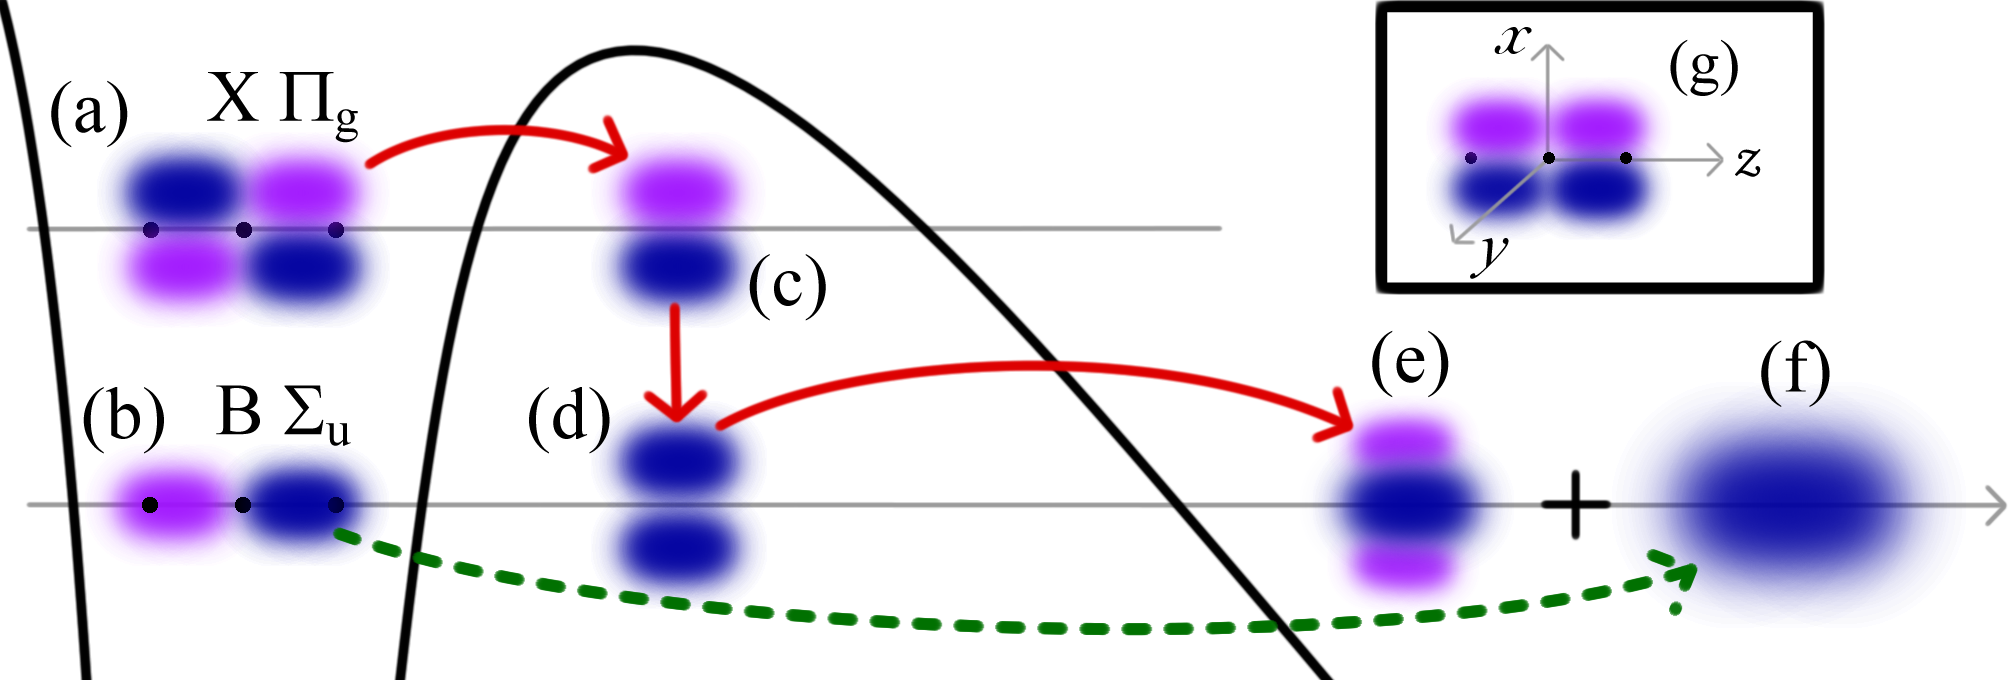
\includegraphics[width=0.75\textwidth]{3-Multi-channel/Figures/figure3C.png}
  \caption[Scheme for the correlation-assisted tunnelling of aligned CO$_2$, with the direct $\B$ channel competing with cross-channel contributions that start in the $\X$ channel.]{
  Correlation-assisted ionization of CO$_2$. An electron can ionize from HOMO~\protect\subref{f3-CO2-X-to-B-coupling-a} and change to an excited channel~\protect\subref{f3-CO2-X-to-B-coupling-b} in a mid-barrier transition~\protect\subref{f3-CO2-X-to-B-coupling-c}. This subjects it~\protect\subref{f3-CO2-X-to-B-coupling-c} to the dipole potential of the transition charge~\protect\subref{f3-CO2-X-to-B-coupling-g}, which changes the relative phase of the two lobes~\protect\subref{f3-CO2-X-to-B-coupling-d}. This double-slit wavefunction then diffracts to multiple lobes~\protect\subref{f3-CO2-X-to-B-coupling-e}. This contrasts to direct ionization on the excited $\B$ channel, which has a single~lobe~\protect\subref{f3-CO2-X-to-B-coupling-f}.
  }
\label{f3-CO2-X-to-B-coupling}
\end{figure}

Here HOMO has a nodal plane along the laser polarization (as does the HOMO$-1$ \mbox{orbital}, $\A\,\Pi_\mathrm{g}$), with two lobes of opposite phase, which means that the outgoing wavepacket inherits this structure and it is also highly suppressed, making $\B\,\Sigma_\mathrm{g}$ a substantial contributor to the ionization, despite its much higher ionization potential~\cite{meckel_LIED_2008, smirnova_multielectron-hhg_2009, mairesse_high-harmonic-spectroscopy_2010}. The position-space node is similarly reflected by a nodal plane at the origin in the momentum-space representation of the electron coming from the $\X$ orbital, embodied in the $R(\vbp)$ shape factor of the previous chapter.

At the moment of the correlation interaction $t''$, which we will integrate over as per Eq.~\eqref{e2-correlation-driven-yield-semi-final}, this wavepacket is impulsively subjected to the correlation potential $\Vnm{\vbr}$, which in this example corresponds to the electrostatic field of the transition charge. This is of the essential form $\braket{\B}{\vbr} \! \braket{\vbr}{\X}$, as depicted in \reffig{f3-CO2-X-to-B-coupling-g}, and since the transition charge is dipolar the potential will essentially be of the form $d_{\B\X}x/r^3$, in the reference frame of \reffig{f3-CO2-X-to-B-coupling-g}, with a node along the same direction as our $\X$-ionized wavepacket.%
\footnote{%
It is important to note, on the other hand, that there is an exactly equivalent channel along the $y$ axis, coming from the $\X\,\Pi_{\mathrm{g},y}$ orbital, which will restore the system's axial symmetry to our result.
}
In momentum space, our linear $\propto x$ potential is therefore proportional to the momentum operator $\frac{\partial}{\partial k_x\!\!\!{}}\,$, and it therefore transforms our two-lobed wavefunction to the three-lobed wavepacket shown in \reffig{f3-CO2-X-to-B-coupling-e}.


The physical picture is most clearly cast in terms of angular momentum. The $\X$ channel is a $\Pi$ state, which means that the outgoing electron and the hole in the core both have angular momenta $L=\pm 1$ about the laser polarization, in opposite directions. The $\B$ channel, on the other hand, is a $\Sigma$ state with zero angular momentum in the core. Inducing an $\X\rightarrow\B$ transition thus requires the outgoing electron to `wind down' the core, returning its angular momentum through the reaction force. This exchange of transverse momentum creates the central lobe.


The lateral lobes in the final momentum distribution are interference effects coming from the interaction region. In position space, the initial tunnelling wavepacket is Gaussian in the transverse direction~\cite{ivanov_anatomy_2005} with a node of the form $\psi\propto x e^{-\frac{1}{2\tau}x^2}$. The impulsive application of the dipole potential transforms it to the form $\psi'\propto x^2 e^{-\frac{1}{2\tau}x^2}$, as depicted in \reffig{f3-CO2-X-to-B-coupling-d}; the final momentum distribution is the Fourier transform of this wavefunction. The situation is then essentially interference from a double slit, formed by the two same-sign lobes of this wavefunction, with three of the fringes visible.










\section{The geometric saddle-point argument}

Having painted an intuitive picture of the process, we now move on to a more formal analysis of the resulting angular distributions. We have built, in chapter~\ref{chap:R-matrix}, most of the machinery we need, in the form of expressions \eqref{e2-ionization-yield-with-shape-factor} for the direct yield and \eqref{e2-correlation-driven-yield-semi-final} for the correlation-assisted contribution, which together~read
\begin{subequations}
\begin{align}
a_n^{(0)}(\vb{p},\tn)
& =
e^{-iE_n\tn}
e^{iI_{p,n} \ts + \frac{i}{2} \int_T^{\ts}\left(\vbp+\vba(\tau)\right)^2\d\tau }
e^{-i\int_\tk^T U_n\left(\int_{ \ts}^\tau \vb{v}(\tau')\d\tau'\right) \d\tau}
R_n(\vbp)
,
\label{e3-direct-yield-recap}
\\
a_n^{(1)}(\vb{p},\tn)
& =
-i 
\sum_m 
e^{-iE_n \tn}
e^{iI_{p,m} \ts}
\int_{\ts}^T\!\d t''
e^{+i(E_n-E_m)t''}
e^{-\frac{i}{2} \int_{t''}^T\left(\vbp+\vba(\tau)\right)^2\d\tau} 
\nonumber \\ & \quad \ \  \times
\frac{1}{(2\pi)^{3}}
\int\!\d\vbk
\int\!\d\vbr \:
\Vnm{\vbr}
R_m(\vbk)
e^{i\left(\vbk-\vbp\right)\cdot\vb{r}} 
e^{-\frac{i}{2} \int_{\ts}^{t''}\left(\vb{k}+\vba(\tau)\right)^2\d\tau} 
e^{-iW_{nm}(\vbr,\vbk,t'')}
.
\label{e3-correlation-driven-yield-recap}
\end{align}
As noted above, one of the main factors that determine these amplitudes is the exponential term in the ionization time, of the form $e^{iI_{p,m} \ts}$, where the imaginary part of the ionization saddle-point time $\ts$ gives the amplitude an exponential dependence on the ionization potential $I_{p,m}$ to the given ionic state. Because of this strong dependence, these contributions will generally be limited to one or a few ionic states, and we therefore break the sum down into its different constituents
\begin{align}
a_{nm}^{(1)}(\vb{p},\tn)
& =
-i
e^{-iE_n \tn}
e^{iI_{p,m} \ts}
\int_{\ts}^T\!\d t''
e^{+i(E_n-E_m)t''}
e^{-\frac{i}{2} \int_{t''}^T\left(\vbp+\vba(\tau)\right)^2\d\tau} 
\nonumber \\ & \quad \quad  \times
\frac{1}{(2\pi)^{3}}
\int\!\d\vbk
\int\!\d\vbr \:
\Vnm{\vbr}
R_m(\vbk)
e^{i\left(\vbk-\vbp\right)\cdot\vb{r}} 
e^{-\frac{i}{2} \int_{\ts}^{t''}\left(\vb{k}+\vba(\tau)\right)^2\d\tau} 
e^{-iW_{nm}(\vbr,\vbk,t'')}
\label{e3-correlation-driven-yield-broken-down}
\end{align}
\end{subequations}
in the understanding that only their full sum, $a_n^{(1)}(\vb{p},\tn) = \sum_m a_{nm}^{(1)}(\vb{p},\tn)$ is of interest. Moreover, since in this chapter we are interested in the geometrical aspects of this amplitude, to which the Coulomb correction $e^{-iW_{nm}(\vbr,\vbk,t'')}$ contributes weakly, we will neglect it for the multi-channel analysis, assuming that it behaves mostly like the single-electron correction which we will examine in chapters \ref{chap:quantum-orbits} and \ref{chap:LES-NZES}.

As we mentioned in the previous chapter, to get a good sense of how the correlation-assisted amplitude \eqref{e3-correlation-driven-yield-broken-down} behaves, it is generally necessary to have explicit values for the interaction potential $\Vnm{\vbr}$ and the initial shape factor $R_m(\vbk)$, since these are crucial ingredients of the geometric integrals over $\vbr$ and $\vbk$. However, there is still more that we can say about the other two factors of the integrand, the exponential terms
\begin{equation}
\exp\left(\vphantom{\int} i\left(\vbk-\vbp\right)\cdot\vb{r} \right)
\exp\left( -\frac{i}{2} \int_{\ts}^{t''}\left(\vb{k}+\vba(\tau)\right)^2\d\tau \right)
,
\label{e3-exponential-factors}
\end{equation}
which also carry a strong dependence on both integration variables.

Moreover, this dependence is rather simple: although it includes an explicit integral over $\tau$, and a variable dependence on $t''$ which will later be integrated over, the exponent in this case is still simply a quadratic function of $\vbk$, which is in general relatively easy to handle. If this quadratic dependence on $\vbk$ (and, as we shall show, later on also on $\vbr$) is sharp enough, we can hope that it will be comparable to the dependence of $R_m(\vbk)$ and $\Vnm{\vbr}$ or faster, and that a saddle-point argument can apply. In any case, it is worthwhile to study this aspect of the structure of the integrand.


This is relatively easy to do, and it amounts to expanding the square in \eqref{e3-exponential-factors}, isolating the integral to powers of $\vba(\tau)$, and completing the square on $\vbk$, which yields
\begin{align}
i\left(\vbk-\vbp\right)\cdot\vb{r}
-\frac{i}{2} \int_{\ts}^{t''}\left(\vb{k}+\vba(\tau)\right)^2\d\tau
& =
-\frac i2 (t''-\ts) (\vbk-\vbk_s(\vbr))^2
-\frac i2 \mathcal{A}^2(t'')
\nonumber \\ & \qquad
+\frac{i/2}{t''-\ts} \left[
  \vbr^2 - 2\vbr \cdot \int_{\ts}^{t''} (\vbp+\vba(\tau))\d\tau  +\bm{\mathcal{A}}(t'')^2
  \right]
\label{e3-completing-squares-k}
\end{align}
in terms of the encapsulated integrals $\bm{\mathcal{A}}(t'')=\int_{\ts}^{t''}\vba(\tau)\d\tau$ and $\mathcal{A}^2(t'')=\int_{\ts}^{t''}\vba(\tau)^2\d\tau$, and the central momentum
\begin{equation}
\vbk_s(\vbr) = \frac{1}{t''-\ts} \left(  \vbr-\int_{\ts}^{t''}\vba(\tau)\d\tau  \right)
.
\label{e3-saddle-point-k}
\end{equation}
Here, however, completing the square with respect to the linear term in $\vbr \cdot \vbk$ now yields a quadratic term in $\vbr$ in the exponent, which also demands to be treated similarly. Thus, completing the square with respect to the central position
\begin{equation}
\vbr_s(\vbp) = \int_{\ts}^{t''} (\vbp+\vba(\tau))\d\tau
\label{e3-saddle-point-r-initial}
\end{equation}
we get
\begin{align}
i\left(\vbk-\vbp\right)\cdot\vb{r}
-\frac{i}{2} \int_{\ts}^{t''}\left(\vb{k}+\vba(\tau)\right)^2\d\tau
& =
-\frac i2 (t''-\ts) (\vbk-\vbk_s(\vbr))^2
+\frac{i/2}{t''-\ts} (\vbr-\vbr_s(\vbp))^2
\nonumber \\ & \qquad
-\frac i2 \int_{\ts}^{t''} (\vbp+\vba(\tau))^2 \d\tau
.
\label{e3-completing-squares-r}
\end{align}


This means, then, that the geometrical integration in \eqref{e3-correlation-driven-yield-broken-down} can be broken down into a sequence of integrals against gaussian-like kernels, as
\begin{align}
a_{nm}^{(1)}(\vb{p},\tn)
& =
-i
e^{-iE_n \tn}
e^{iI_{p,m} \ts}
\int_{\ts}^T\!\d t''
e^{+i(E_n-E_m)t''}
e^{-\frac{i}{2} \int_{t''}^T\left(\vbp+\vba(\tau)\right)^2\d\tau} 
e^{-\frac i2 \int_{\ts}^{t''} (\vbp+\vba(\tau))^2 \d\tau}
\nonumber \\ & \quad \quad  \times
\frac{1}{(2\pi)^{3}}
\int\!\d\vbr \:
e^{\frac{i/2}{t''-\ts} (\vbr-\vbr_s(\vbp))^2}
\Vnm{\vbr}
\int\!\d\vbk
e^{-\frac i2 (t''-\ts) (\vbk-\vbk_s(\vbr))^2}
R_m(\vbk)
\label{e3-correlation-driven-yield-with-completed-squares}
\end{align}
where, moreover, the $\vbp$-dependent phases come together into a single $t''$-independent integral identical to the factor in \eqref{e3-direct-yield-recap}, giving
\begin{align}
a_{nm}^{(1)}(\vb{p},\tn)
& =
-i
e^{-iE_n \tn}
e^{iI_{p,m} \ts+\frac{i}{2} \int_T^{\ts}\left(\vbp+\vba(\tau)\right)^2\d\tau} 
\int_{\ts}^T\!\d t''
e^{+i(E_n-E_m)t''}
\nonumber \\ & \quad \times
\frac{1}{(2\pi)^{3}}
\int\!\d\vbr \:
e^{\frac{i/2}{t''-\ts} (\vbr-\vbr_s(\vbp))^2}
\Vnm{\vbr}
\int\!\d\vbk  \:
e^{-\frac i2 (t''-\ts) (\vbk-\vbk_s(\vbr))^2}
R_m(\vbk)
.
\label{e3-correlation-driven-yield-with-completed-squares-2}
\end{align}


Here is where the saddle-point argument comes in. If the molecular geometrical factors $R_m(\vbk)$ and $\Vnm{\vbr}$ are relatively slow compared to the two exponentials, which is generally the case, then we are justified in considering them as constant and doing the gaussian integrals explicitly. In that case, then, the momentum integral evaluates as
\begin{equation}
\int\!\d\vbk  \:
e^{-\frac i2 (t''-\ts) (\vbk-\vbk_s(\vbr))^2}
R_m(\vbk)
=
\left(
 \frac{2\pi}{i(t''-\ts)}
 \right)^{3/2}
R_m(\vbk_s(\vbr))
,
\label{e3-geometric-integral-after-k-spa}
\end{equation}
and this feeds into the position integral to give the remarkable simple result
\begin{align}
\frac{1}{(2\pi)^{3}}
&
\int\!\d\vbr \:
e^{\frac{i/2}{t''-\ts} (\vbr-\vbr_s(\vbp))^2}
\Vnm{\vbr}
\left(
 \frac{2\pi}{i(t''-\ts)}
 \right)^{3/2}
R_m(\vbk_s(\vbr))
%
\nonumber \\ & \qquad =
%
\frac{1}{(2\pi)^{3}}
\left(
 \frac{2\pi}{i(t''-\ts)}
 \right)^{3/2}
\left(
 \frac{2\pi}{-i/(t''-\ts)}
 \right)^{3/2}
\Vnm{\vbr_s(\vbp)}
R_m(\vbk_s(\vbr_s(\vbp)))
%
\nonumber \\[5pt] & \qquad =
%
\Vnm{\vbr_s(\vbp)}
R_m(\vbk_s(\vbr_s(\vbp)))
.
\label{e3-geometrical-saddle-point-simplified}
\end{align}


One notable aspect of this development is that the saddle-point momentum (which, regardless of the validity of the geometrical saddle-point approximation, is where the two gaussian factors are concentrated) simplifies rather drastically, and it simplifies to
\begin{align}
\vbk_s(\vbr_s(\vbp)) 
& = 
\frac{1}{t''-\ts} \left(  \vbr_s(\vbp)-\int_{\ts}^{t''}\vba(\tau)\d\tau \right)
\nonumber \\ & = 
\frac{1}{t''-\ts} \left(  \int_{\ts}^{t''} (\vbp+\vba(\tau))\d\tau - \int_{\ts}^{t''}\vba(\tau)\d\tau  \right)
\nonumber \\ & = 
\vbp
,
\end{align}
that is, to the final measured momentum. More physically, this states that, within the approximations we have used, the Coulomb correlation interaction via $\Vnm{\vbr}$ between the photoelectron and the ionic core does not change the photoelectron's momentum or its kinetic energy, regardless of whether it is still under the tunnelling barrier or already outside it, but it does change the final energetic state of the ion.

(This is, of course, an approximation as far as the energy conservation law is concerned, and it is valid when $\Delta I_p\ll I_p$. Then, the modification of the outgoing trajectory is small, and the paradox is somewhat reduced. This approximation is well justified, since if $\Delta I_p$ is large then the highest-lying molecular orbital will completely dominate the ionization.)

To make this somewhat more explicit, under the geometric saddle-point approximation the correlation-driven yield reduces to the form
\begin{align}
a_{nm}^{(1)}(\vb{p},\tn)
& =
-i
e^{-iE_n \tn}
e^{iI_{p,m} \ts+\frac{i}{2} \int_T^{\ts}\left(\vbp+\vba(\tau)\right)^2\d\tau} 
R_m(\vbp)
\int_{\ts}^T\!
e^{+i(E_n-E_m)t''}
\Vnm{\rl(t'')}
\d t''
,
\label{e3-correlation-driven-yield-after-geometric-SPA}
\end{align}
which splits into a prefactor exactly equal to the direct yield \eqref{e3-direct-yield-recap} (aside from Coulomb factors, which we're neglecting in this chapter) and a temporal integral over the interaction, where we have re-labelled the position saddle point as
\begin{equation}
\rl(t) = \int_{\ts}^{t} [\vbp+\vba(\tau)]\d\tau,
\label{e3-laser-driven-trajectory}
\end{equation}
the laser-driven trajectory that starts at the origin at complex time $\ts$ and has asymptotic momentum $\vbp$. In this form, \eqref{e3-correlation-driven-yield-after-geometric-SPA} now requires explicit integration over the interaction time $t''$ of the correlation interaction potential $\Vnm{\rl(t'')}$, so in general this will have to be done numerically once a specific potential and momentum are fixed.






\section{A solvable model}
In general, the saddle-point analysis just presented works fairly well, but it is concerning that the shape factor of the direct-tunnelling process, $R_m(\vbp)$, is retained intact without any change in the central momentum $\vbk_s=\vbp$, in a process which should deliver some form of momentum kick to the outgoing photoelectron when it interacts with the ionic core on its way out. 

There is, then, some tension between the physical expectation of a more specific change in the photoelectron's momentum and the mathematical expectation that, for reasonable orbital shape factors $R_m(\vbk)$ and correlation interaction potentials $\Vnm{\vbr}$, the saddle-point approximation should work well. This tension motivated, in previous work reported in the author's MRes report~\cite{MResReport}, an explicit calculation using reasonable multipolar models for both the shape factor and the interaction potential. If one compares those results with the ones from the saddle-point argument, a painful fact appears: the saddle-point approximation can fail, and rather loudly so, in this situation.

The explicit calculation of \citer{MResReport} will not be repeated here, as it is rather technical and space-intensive. Instead, this section will develop a simple toy model -- a thoroughly boiled down version of the full calculation -- for which the geometric integrals of \eqref{e3-correlation-driven-yield-broken-down} can be integrated explicitly to a result that disagrees with the saddle-point result. Moreover, this result completely encapsulates the reasons for this disagreement. As such, this toy model allows us to decide in what situations the geometrical saddle-point approximation is valid, and it points to how to fix it when it breaks. 

In terms of actual calculations for real molecules, the correlation potentials integrated over in \eqref{e3-correlation-driven-yield-after-geometric-SPA} and its modifications must be taken from quantum chemical calculations, and we will examine in chapter \ref{chap:complex-space-potentials} what happens when we require those potentials at the complex positions demanded by the laser-driven trajectory \eqref{e3-laser-driven-trajectory}, which does impose nontrivial restrictions. Nevertheless, in general it is not necessary to resort to the model potentials of \citer{MResReport} for calculations, and the simplified toy model we develop here offers an easier insight into why the geometrical saddle-point calculations need to be modified.

In short, the failure of the geometrical saddle-point approximation for \eqref{e3-correlation-driven-yield-broken-down} occurs when it predicts a zero or near-zero result, through a zero of $R_m(\vbk)$, $\Vnm{\vbr}$ or more usually both. In those conditions, the saddle-point approximation -- in reality, the leading term of an asymptotic series -- becomes comparable with, or smaller than, the sub-leading term of that series, so both terms need to be included. Doing this then returns the approximation to excellent agreement.



To appropriately model these zeroes, we refer explicitly for our toy model to the transition we chose, the $\X\to\B$ transition in CO$_2$ aligned along the laser polarization, as shown earlier in \reffig{f3-CO2-X-to-B-coupling}. In this configuration, the initial $\X\:\Pi_\mathrm{g}$ orbital has a node along the laser polarization, so its shape factor is of the form
\begin{equation}
R_m(\vbk)=C_m(k_z)k_x = \frac{C_{0,m}}{\sqrt{iS_V''(\ts)}}k_x.
\end{equation}
The correlation interaction potential, on the other hand, as defined in \eqref{e2-Vnm-definition}, is caused by the overlap density between the $\X$ and $\B$ orbitals, shown in \reffig{f3-CO2-X-to-B-coupling-g}, which as we argued earlier must also have a node along the laser polarization. The simplest model, then is a dipolar interaction, so we take
\begin{equation}
\Vnm{\vbr}=\frac{d_{mn}x}{(z^2+\sigma^2)^{3/2}}.
\end{equation}
This is a standard dipolar interaction, going down as $1/r^3$, where we've replaced $r$ by the longitudinal coordinate $z$ for simplicity and to reflect the generally small angle of ionization, and we've added a softening by $\sigma$ to account for the finite size of the molecular dipole charge. This potential does not account for all of the true potential's spatial variation, but it captures the essence that interests us in this chapter.


We can now put in these explicit factors into the geometrical factors of the correlation-assisted yield \eqref{e3-correlation-driven-yield-broken-down}, and this gives us
\begin{align}
I_\mathrm{geom}
& =
\frac{1}{(2\pi)^{3}}
\int\!\d\vbk
\int\!\d\vbr \:
\Vnm{\vbr}
R_m(\vbk)
e^{i\left(\vbk-\vbp\right)\cdot\vb{r}} 
e^{-\frac{i}{2} \int_{\ts}^{t''}\left(\vb{k}+\vba(\tau)\right)^2\d\tau} 
\nonumber \\ & =
\frac{1}{(2\pi)^{3}}
\int\!\d\vbk
\int\!\d\vbr \:
\frac{d_{mn}x}{(z^2+\sigma^2)^{3/2}}
C_m(k_z)k_x
e^{i\left(\vbk-\vbp\right)\cdot\vb{r}} 
e^{-\frac{i}{2} \int_{\ts}^{t''}\left(\vb{k}+\vba(\tau)\right)^2\d\tau} 
\nonumber \\ & =
I_x I_y I_z
,
\end{align}
a well-defined geometrical integral that can now be tackled directly, and which moreover splits cleanly into component parts.

From these, the $y$ component is essentially trivial, since at
\begin{equation}
I_y
=
\frac{1}{2\pi}
\int \! \d k_y \! \int \! \d y \:
e^{i(k_y-p_y)y}
e^{-\frac{i}{2} (t''-\ts)k_y^2}
\end{equation}
it is a pair of simple gaussian integrals, so the saddle-point result is exact, giving $I_y=1$ as per \eqref{e3-geometrical-saddle-point-simplified}. Similarly, the longitudinal $z$ component can generally be well approximated by the saddle-point integration, as long as $C_m(k_z)$ is slow enough, in which case that integral~reads
\begin{align}
I_z
& =
\frac{1}{2\pi}
\int \! \d k_z \! \int \! \d z \:
\frac{C_m(k_z)}{(z^2+\sigma^2)^{3/2}}
e^{i(k_x-p_x)x}
e^{-\frac{i}{2} \int_{\ts}^{t''}\left(k_z+A_z(\tau)\right)^2\d\tau}
\nonumber \\ & =
\frac{C_m(p_z)}{(z(t'')^2+\sigma^2)^{3/2}}
e^{-\frac{i}{2} \int_{\ts}^{t''}\left(p_z+A_z(\tau)\right)^2\d\tau}
,
\end{align}
exactly analogously to the previous case.


The problem, as expected, is in the $x$ part of the geometrical integral, since this is the direction where we have put both of the relevant nodes, in $x$ and in $k_x$:
\begin{equation}
I_x
=
\frac{1}{2\pi}
\int \! \d k_x \! \int \! \d x \:
d_{mn}x k_x
e^{i(k_x-p_x)x}
e^{-\frac{i}{2} (t''-\ts)k_x^2}
.
\end{equation}
This is, again, pretty close to a gaussian integral, and it can be done exactly. In fact, for the first step of integration, over $k_x$, the saddle-point method is again exact, since the prefactor splits as
\begin{equation}
k_x=(k_x-k_x^{(s)})+k_x^{(s)},
\end{equation}
where the first term is odd about $k_x^{(s)}$ and gives a zero integral with respect to the even gaussian kernel, leaving only the constant term at the saddle point. Splitting the exponent as in \eqref{e3-completing-squares-r}, then, gets us
\begin{align}
I_x
& =
\frac{d_{mn}}{2\pi}
e^{-\frac{i}{2} (t''-\ts)p_x^2}
\int 
\d x \,
x \,
e^{\frac{i/2}{t''-\ts}\left(x-x^{(s)}\right)^2}
\int 
\d k_x \,
k_x\,
e^{-\frac{i}{2} (t''-\ts)\left(k_x-k_x^{(s)}\right)^2} 
\nonumber \\ & =
\frac{d_{mn}}{2\pi}
\left(
 \frac{2\pi}{i(t''-\ts)}
 \right)^{1/2}
e^{-\frac{i}{2} (t''-\ts)p_x^2}
\int 
x \,
k_x^{(s)} \,
e^{\frac{i/2}{t''-\ts}\left(x-x^{(s)}\right)^2}
\d x
,
\label{e3-Ix-integral-after-k-integration}
\end{align}
where the saddle point as per \eqref{e3-saddle-point-k} is given by $k_x^{(s)}= x/(t''-\ts)$, so the integral is given~by
\begin{align}
I_x
& =
\frac{d_{mn}}{2\pi}
\left(
 \frac{2\pi}{i(t''-\ts)}
 \right)^{1/2}
\frac{
 e^{-\frac{i}{2} (t''-\ts)p_x^2}
 }{t''-\ts}
\int 
x^2 \,
e^{\frac{i/2}{t''-\ts}\left(x-x^{(s)}\right)^2}
\d x
\label{e3-Ix-integral-with-x2-node}
\end{align}
with a saddle point at $x^{(s)}=(t''-\ts)p_x$.

Here, finally, lies the root of the failure of the saddle-point approximation for the geometrical integrals, at the failure of the approximation for integrals of the form
\begin{equation}
\int 
x^2 \,
e^{\frac{i/2}{t''-\ts}\left(x-x^{(s)}\right)^2}
\d x
.
\end{equation}
At low transverse momenta, $p_x\approx 0$, the saddle point $x^{(s)}=(t''-\ts)p_x$ is very close to the quadratic zero of the prefactor at $x=0$, which means that the saddle-point approximation when taken naively will yield a zero value for the integral. However, even at $p_x=x^{(s)}=0$, the area under the curve $x^2e^{-x^2}$, shown in \reffig{f3-gaussian-with-node}, is simply not zero.


\begin{figure}[htb]
  \centering
  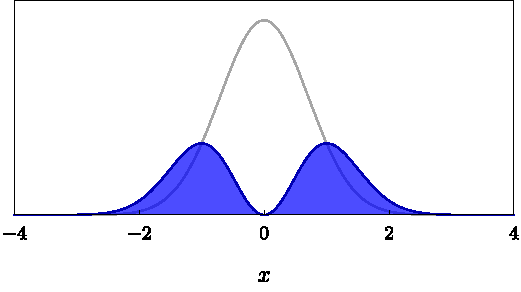
\includegraphics[scale=1]{3-Multi-channel/Figures/figure3A.pdf}
  \caption[Plots of $e^{-x^2}$ and $x^2e^{-x^2}$ as functions of $x$]{Plots of $e^{-x^2}$ and $x^2e^{-x^2}$ as functions of $x$, with the (nonzero) area under the latter shaded in blue.}
  \label{f3-gaussian-with-node}
\end{figure}



This simply means, of course, that the saddle-point approximation needs to be modified to take explicit care of this possibility. In its usual form, approximating an integral of the form $\int_A^B F(\zeta) e^{\rho \varphi(\zeta)} \d\zeta$ by the value $F(\zeta_s) e^{\rho\varphi(\zeta_s)}$ of its integral at the saddle point $\zeta_s$ comes from neglecting the spatial variation of $F(\zeta)$ near the saddle point, i.e., from replacing it with its zeroth-order Taylor expansion there. For cases like $x^2e^{-x^2}$, one simply needs to take an appropriate number of terms in the Taylor series, which -- like $\int x^2 e^{-x^2} \d x$ -- can also be integrated exactly.






\begin{mathaside}{The saddle-point approximation for saddle points near zeros of the prefactor}
\label{aside.SPAreprise}
\noindent
To make this more precise in general, consider again  an analytic function $F$ which varies slowly with respect to the analytic exponent $\varphi$, integrated as $\int_A^B F(\zeta) e^{\rho \varphi(\zeta)}\d\zeta$ over a contour that includes a single saddle point $\zeta_s$ such that $\varphi'(\zeta_s)=0$. Taking an $N$-term Taylor expansion for $F$, and the leading-order expansion for $\varphi$, at $\zeta_s$ gives an expansion of the form
\begin{equation}
\int_A^B F(\zeta) e^{\rho \varphi(\zeta)}\d\zeta
\approx
\sum_{n=0}^{2N}\frac{F^{(n)}(\zeta_s)}{n!}  e^{\rho \varphi(\zeta_s)}\int_A^B (\zeta-\zeta_s)^n  e^{\frac12 \rho \varphi ''(\zeta_s)(\zeta-\zeta_s)^2} \d\zeta
,
\end{equation}
with only the leading order term in the expansion of $\varphi$ contributing because of the exponential effect of a large $\rho$.

\vspace{\maskip}
In this expansion, all the odd powers of $\zeta-\zeta_s$ disappear, because they give an integrand of odd overall symmetry about $\zeta_s$, leaving only the even terms of the form $\zeta^{2n}e^{-\zeta^2}$ integrated over a contour which (in the asymptotic regime of~$\rho\to\infty$) is much longer than the dimensions of the gaussian envelope. Extending the contour to infinity, the integrals can then be performed exactly~\cite{BruijnAsymptotics, GerlachSPAonline}, and this gives the approximation
\begin{equation}
\int_A^B F(\zeta) e^{\rho \varphi(\zeta)}\d\zeta
\approx
\sqrt{\frac{2\pi}{\rho}} 
\frac{e^{\rho\varphi(\zeta_s)}}{\left[-\varphi''(\zeta_s)\right]^{1/2}}
\sum_{n=0}^N
\frac{(-1)^n}{n!}
\frac{
  F^{(2n)}(\zeta_s) 
  }{
  \left(2\rho\varphi''(\zeta_s)\right)^n
  }
.
\label{e3-full-SPA-statement}
\end{equation}

In general, the Taylor series should not be taken to too high a degree $N$, as this would push the relevant contributions too far from the saddle point and closer to points where the ends of the contour, or other saddles, could interfere. In a formal sense, the approximation \eqref{e3-full-SPA-statement} only works as an asymptotic series, in which more terms can only be included when the asymptotic parameter $\rho$ is large~enough. 

For our purposes, though, this expansion serves its purpose at the leading-term level, except when the prefactor is too small at the saddle point, in which case only one or two additional terms need to be included.
\end{mathaside}


Coming back to our integral, we now see that the saddle-point approximation is again exact -- if taken to the second order, which is of course the exact integration we want. Thus, we have
\begin{equation}
\int 
x^2 \,
e^{\frac{i/2}{t''-\ts}\left(x-x^{(s)}\right)^2}
\d x
=
\left(
 \frac{2\pi}{-i/(t''-\ts)}
 \right)^{1/2}
\left(
\left(x^{(s)}\right)^2 + i (t''-\ts)
\right)
,
\end{equation}
where the quadratic term in $x^{(s)}\propto p_x$ is the usual saddle-point contribution, which is dominated at low $p_x$ by the second-order term, a constant with respect to $p_x$. Putting in this integral into $I_x$, then, we have the exact expression
\begin{align}
I_x
& =
i d_{mn}
e^{-\frac{i}{2} (t''-\ts)p_x^2}
\left(  1 - i(t''-\ts)p_x^2  \right)
e^{-\frac{i}{2} (t''-\ts)p_x^2}
,
\label{e3-Ix-final}
\end{align}
and this is what determines the angular profile of the correlation-driven wavefunction for this geometry.


Here there are several observations worth making. The first is that the angular distribution for this cross-channel is indeed very different to what we would have obtained using the direct saddle-point argument, as shown in \reffig{f3-angular-distribution-plots}. The angular profile for this channel now has a nontrivial structure with sign changes across the distribution, and this would not be obtained otherwise. Moreover, the angular structure of the cross channel is distinct from that of the direct channel, so their final interference -- at amplitudes and phases still to be determined -- will in general also have an interesting angular variation.


\begin{figure}[htb]
  \centering
  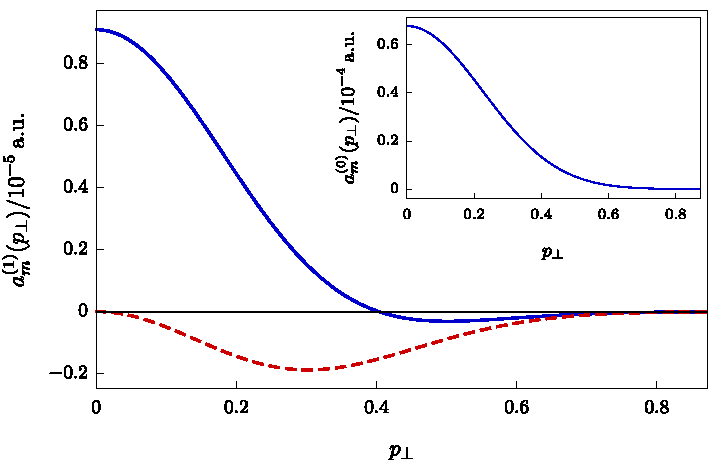
\includegraphics[scale=1]{3-Multi-channel/Figures/figure3D.pdf}
  \caption[Transverse ionization spectra for aligned CO$_2$, coming from the direct and correlation-driven channels, as well as the geometrical saddle-point approximation to the latter]{
  Momentum-resolved ionization yield for the $\X\to\B$ perpendicular dipole transition in parallel-aligned CO$_2$, with the corresponding direct amplitude in the inset. The dashed curve is the prediction from the spatial saddle-point approximation.
  The parameters used are $F=\SI{0.05}{\au}$ and $\omega=\SI{0.057}{\au}$ (so $I=\SI{9e13}{W/cm^2}$ and $\lambda=\SI{800}{nm}$), $d_{\B\X}=\SI{0.175}{\au}$, $\sigma=\SI{2.19}{\au}$, $C_{0,\X}=\SI{0.23}{\au}$, $C_{0,\B}=\SI{0.18}{\au}$, $I_{p,\X}=\SI{0.5064}{\au}$, and $I_{p,\X}=\SI{0.6644}{\au}$
  }
  \label{f3-angular-distribution-plots}
\end{figure}


Somewhat more physically, it is important to remark that the central lobe of \reffig{f3-angular-distribution-plots} is purely a wave phenomenon, caused by the Fourier transformation, via $e^{ip_xx}$, of the gaussian-with-a-hole wavefunction that results from taking the two-lobed gaussian that results from the direct tunnelling in the initial channel, of the form $k_x e^{-\Delta t k_x^2}$, and multiplying it by a transition operator proportional to $\Vnm{\vbr}\propto x$. That is, as tunnelling goes on, the wavefunction forms in position space in the form $x^2 e^{ix^2/\Delta t}$, and this looks (since $\Delta t$ is imaginary) much like the function in \reffig{f3-gaussian-with-node}. In essence, this is a double-slit wavefunction, as depicted in \reffig{f3-CO2-X-to-B-coupling}, and the momentum distribution determined by \eqref{e3-Ix-final} is precisely the far-field diffraction pattern caused by this double slit. To make this a bit more interesting, though, since the pattern forms primarily while $t''$ is still complex and the photoelectron is still inside the tunnelling barrier, the far-field angular distribution shown in \reffig{f3-angular-distribution-plots} is a diffraction pattern that originates from a matter-wave double slit that occurs inside a tunnelling~barrier, as shown in the step from \subref{f3-CO2-X-to-B-coupling-d} to \subref{f3-CO2-X-to-B-coupling-e} in \reffig{f3-CO2-X-to-B-coupling}.









\section{Modified saddle-point arguments for real molecules}
As we have seen, the saddle-point approximation can fail when compared to exact calculations for toy models of experimentally relevant geometries. Unfortunately, the route of exact calculation faces a rather steep uphill climb if it is to describe realistic molecules. One such example is the calculation in \citer{MResReport}, which models the molecule via relatively simple descriptors of the form
\begin{equation}
R_m(\vbk)=C(k_z)e^{im_1\phi_k}k_\perp^{|m_1|}
\quad \text{and} \quad
\Vnm{\vbr}=\frac{Q_{\ell m_2}}{r^{\ell+1}}Y_{\ell m_2}(\theta, \phi)
,
\end{equation}
and still only obtains a result in series form. For a realistic molecule, this is an unsatisfactory model because in the neighbourhood of the molecule the presence of ionic electrons makes the correlation interaction potential $\Vnm{\vbr}$ a solution of the Poisson (rather than the Laplace) equation. Moreover, obtaining a good model for a given molecule in terms of multipolar potentials is not particularly easy. Other analytically integrable models are also possible, but they also present significant challenges.

In general, the electronic structure of the remaining ion -- the ionic states $\{\ket{n}\}$ and the properties that emanate from them -- is a problem for quantum chemistry, and indeed the discipline has much to say on the subject of our correlation interaction potential $\Vnm{\vbr}$. While the numerical, quantum chemical evaluation of $\Vnm{\vbr}$ is still the cleanest and simplest way to the quantity, unfortunately there are some rather fundamental difficulties and limitations to computing this quantity when it is queried at the complex trajectories that interest us, which we will explore in chapter \ref{chap:complex-space-potentials}.

In this paradigm, of course, exact analytical integration of the geometrical integrals is ruled out, since $\Vnm{\vbr}$ can only be queried numerically. This is a reasonable solution in the saddle-point approximation in which \eqref{e3-correlation-driven-yield-with-completed-squares-2} is reduced to \eqref{e3-correlation-driven-yield-after-geometric-SPA} giving
\begin{align}
a_{nm}^{(1)}(\vb{p},\tn)
& =
-i
e^{-iE_n \tn}
e^{iI_{p,m} \ts+\frac{i}{2} \int_T^{\ts}\left(\vbp+\vba(\tau)\right)^2\d\tau} 
\int_{\ts}^T\!\d t''
e^{+i(E_n-E_m)t''}
\nonumber \\ & \quad \times
\frac{1}{(2\pi)^{3}}
\int\!\d\vbr \:
e^{\frac{i/2}{t''-\ts} (\vbr-\vbr_s(\vbp))^2}
\Vnm{\vbr}
\int\!\d\vbk  \:
e^{-\frac i2 (t''-\ts) (\vbk-\vbk_s(\vbr))^2}
R_m(\vbk)
\nonumber \\ & \approx
-i
e^{-iE_n \tn}
e^{iI_{p,m} \ts+\frac{i}{2} \int_T^{\ts}\left(\vbp+\vba(\tau)\right)^2\d\tau} 
\int_{\ts}^T\!
R_m(\vbp)
\Vnm{\rl(t'')}
e^{+i(E_n-E_m)t''}
\d t''
,
\end{align}
since here $\Vnm{\vbr}$ only needs to be queried at a limited set of positions for the temporal integration. As we've seen, though, this direct saddle-point approximation is flawed, but the roots of the flaw are clear and it can be fixed by suitable modifications of the saddle-point approximation. Doing this then permits us to perform the temporal integral over $t''$ with only one (or a few) evaluations of $\Vnm{\vbr}$ per temporal integration point.


To reformulate the geometrical saddle-point method, then, we need to look for the quadratic zeros of the $\vbr$ and $\vbk$ integrand. In general, though, we can be rather more specific than that, since if only $p$ orbitals are involved, with linear nodes at most, then the emergence of zeroes is always as in \eqref{e3-Ix-integral-after-k-integration} and \eqref{e3-Ix-integral-with-x2-node}, with linear nodes in both factors combining to make a more complicated quadratic zero. In terms of our previous development, this means that we can interrupt the saddle-point method just after the $\vbk$ integration of \eqref{e3-geometric-integral-after-k-spa}, at which point the ionization yield reads

\begin{align}
a_{nm}^{(1)}(\vb{p},\tn)
& =
-i
e^{-iE_n \tn}
e^{iI_{p,m} \ts+\frac{i}{2} \int_T^{\ts}\left(\vbp+\vba(\tau)\right)^2\d\tau} 
\int_{\ts}^T\!\d t''
e^{+i(E_n-E_m)t''}
\nonumber \\ & \quad \times
\frac{1}{(2\pi)^{3}}
\left(
 \frac{2\pi}{i(t''-\ts)}
 \right)^{3/2}
\int\!\d\vbr \:
\Vnm{\vbr}
R_m(\vbk_s(\vbr))
e^{\frac{i/2}{t''-\ts} (\vbr-\vbr_s(\vbp))^2}
.
\label{e3-correlation-driven-yield-reprise-after-k-integral}
\end{align}


Here, then, we apply our extended saddle-point approximation \eqref{e3-full-SPA-statement}, going to second order in the derivatives of the prefactor. In contrast to our original development of the approximation, though, here we have multiple dimensions to handle, so taking the subleading terms should be interpreted as taking only the second derivative in each dimension and adding them up (i.e., ignoring terms of the form $\frac{\partial^2\varphi}{\partial x^2} \frac{ \partial^2 \varphi}{\partial y^2}$), which cleanly yields a rotation-invariant Laplacian of the $\vbr$-dependent prefactor.

This means, then, that our previous \eqref{e3-geometrical-saddle-point-simplified} should be reformulated to read

\begin{align}
\frac{1}{(2\pi)^{3}}
&
\left(
 \frac{2\pi}{i(t''-\ts)}
 \right)^{3/2}
\int\!\d\vbr \:
\Vnm{\vbr}
R_m(\vbk_s(\vbr))
e^{\frac{i/2}{t''-\ts} (\vbr-\vbr_s(\vbp))^2}
%
\nonumber \\ & \quad =
%
\frac{1}{(2\pi)^{3}}
\left(
 \frac{2\pi}{i(t''-\ts)}
 \right)^{3/2}
\left(
 \frac{2\pi}{-i/(t''-\ts)}
 \right)^{3/2}
\times
%
\nonumber \\ & \quad \quad \times
%
\left[
 \Vnm{\vbr_s(\vbp)}
 R_m(\vbk_s(\vbr_s(\vbp)))
 +
 \frac{i}{2} (t''-\ts)
 \nabla_{\vbr}^2
 \left(
   \vphantom{\sum}
   \Vnm{\vbr}
   R_m(\vbk_s(\vbr))
 \right)_{\vbr_s(\vbp)}
\right]
%
\nonumber \\[3pt] & \quad =
%
\Vnm{\vbr_s(\vbp)}
R_m(\vbk_s(\vbr_s(\vbp)))
 +
 \frac{i}{2} (t''-\ts)
 \nabla_{\vbr}^2
 \left(
   \vphantom{\sum}
   \Vnm{\vbr}
   R_m(\vbk_s(\vbr))
 \right)_{\vbr_s(\vbp)}
.
\label{e3-geometrical-saddle-point-reprise-r}
\end{align}
%
%
Moreover, here the second derivative that acts on the product $\Vnm{\vbr} R_m(\vbk_s(\vbr))$ really only needs to pick out the cross terms that arise from the conjunction of linear zeroes in each factor. As such, it can generally be simplified to the form
\begin{align}
\nabla_{\vbr}^2
\left(
  \vphantom{\sum}
  \Vnm{\vbr}
  R_m(\vbk_s(\vbr))
\right)
%
& \approx
%
2 \left( \nabla_{\vbr}\Vnm{\vbr} \right)
\cdot
\left( \nabla_{\vbr} R_m(\vbk_s(\vbr)) \right)
%
\nonumber \\ & =
%
\frac{2}{t''-\ts} 
\left( \nabla_{\vbr}\Vnm{\vbr} \right)
\cdot
\left( \nabla_{\vbk} R_m(\vbk_s(\vbr)) \right)
\end{align}
with the factor of $t''-\ts$ coming from the derivative of $\vbk_s(\vbr)$ with respect to $\vbr$ as per \eqref{e3-saddle-point-k}. Putting this approximation into \eqref{e3-geometrical-saddle-point-reprise-r} then gives us


\begin{align}
\frac{1}{(2\pi)^{3}}
&
\left(
 \frac{2\pi}{i(t''-\ts)}
 \right)^{3/2}
\int\!\d\vbr \:
\Vnm{\vbr}
R_m(\vbk_s(\vbr))
e^{\frac{i/2}{t''-\ts} (\vbr-\vbr_s(\vbp))^2}
%
\nonumber \\ & \quad \approx
%
\Vnm{\vbr_s(\vbp)}
R_m(\vbk_s(\vbr_s(\vbp)))
+
i
\nabla_{\vbr}\Vnm{\vbr_s(\vbp)}
\cdot
\nabla_{\vbk} R_m(\vbk_s(\vbr_s(\vbp))) 
\label{e3-geometrical-saddle-point-with-explicit-grad-dot-grad}
\end{align}
for the geometrical integrals, and 
\begin{align}
a_{nm}^{(1)}(\vb{p},\tn)
& =
-i
e^{-iE_n \tn}
e^{iI_{p,m} \ts+\frac{i}{2} \int_T^{\ts}\left(\vbp+\vba(\tau)\right)^2\d\tau} 
\int_{\ts}^T\!\d t''\:
e^{+i(E_n-E_m)t''}
\nonumber \\ & \qquad \quad \times
\left(
\vphantom{\sum}
\Vnm{\rl(t'')}
R_m(\vbp)
+
i
\nabla_{\vbr}\Vnm{\rl(t'')}
\cdot
\nabla_{\vbp} R_m(\vbp) 
\right)
.
\label{e3-correlation-driven-yield-reprise-with-full-derivatives}
\end{align}
for the final correlation-driven yield.

This expression, then, addresses the failures of the saddle-point approximation clearly exhibited by the toy model, while still retaining the simplicity and numerical ease afforded by the saddle-point method. Here we are spared the need for a full $\vbr$ integration at each time step, and instead we require only a single evaluation of $\Vnm{\vbr}$ and one of its derivatives, $\nabla_{\vbr}\Vnm{\vbr}$. Moreover, depending on the method used to calculate $\Vnm{\vbr}$, the calculation of the gradient can be relatively cheap, when done numerically, and it can even fall out essentially for free from the same quantum chemical calculations that yield the potential.

















